\chapter{超新星遗迹和磁流体相关理论}
\label{Theory}

\section{超新星遗迹激波加速和宇宙线}
\label{TheoryDSACR}
二战结束后,很多用于军事的射电观测设备和技术被应用于天文探索,而这段时间观测发现银河系内
存在很多非热射电源。
\citet{1953AZh....30...15S}首次提出这些非热辐射源自于过去爆发却未被看到的超新星的残骸,
而辐射机制就是同步辐射。
这一猜测随着观测的增多逐步得到证实,直到今天,射电观测仍然是证认SNR的重要手段,而截至
目前,我们已经观测到300多个SNR\citep{2014BASI...42...47G}。

同步辐射产生SNR的非热谱有一个前提,就是辐射电子是相对论化且幂律分布的
\citep{1970ranp.book.....P}。
\citet{Fermi1949}提出的宇宙线加速机制刚好使得电子可以满足这一前提,同时也提到了超新星
爆发或者SNR演化或许会引起这样的加速。
\citet{1953AZh....30...15S}也是以此为依据提出同步辐射机制产生SNR中的射电辐射。
Fermi其实更多是想解释观测到的宇宙线能谱,因为当时逐渐受到关注的宇宙线观测显示其能谱是
幂律谱,这就需要一个加速机制解释这件事,所以他只是提出了一个能产生幂律谱的机制,并没有
深入阐述这个机制如何在SNR中起作用。
这主要是个将磁化云块作为磁镜的机制,因为粒子接近云块加速远离云块减速,所以互相抵消,结果
加速效率与云块的速度和粒子的速度比率的二次方成正比,我们称之为费米二阶加速机制。
很快,有人注意到这个机制的加速效率过低,不足以解释观测结果,并尝试寻找更高效的加速机制。
同时,人们意识到,强激波中的加速可以实现只有粒子接近云块的加速过程,而没有离开云块的减速
过程,这样加速效率与云块的速度和粒子的速度比率的一次方成正比,我们称之为费米一阶
加速机制,又称扩散激波加速机制(Diffusive Shock Acceleration, DSA)
\citep{1977ICRC...11..132A,1977SPhD...22..327K,Bell1978,Blandford1978}。
通常,我们所说的费米加速机制主要就是指费米一阶加速,也就是DSA。

\subsection{扩散激波加速机制}
我们知道,物体在介质中进行超音速运动就会形成激波。
而在SNR中,所谓的介质就是ISM,而超音速运动的物体就是超新星爆发的抛射物。
抛射物挤压ISM,导致ISM在抛射物前方堆积,形成激波面。
也就是说,抛射物与激波面虽然很近,但是还有一定距离,类似于超音速飞机与其前方激波的关系。
通常理想气体介质中的声速$c_s$可以由$c_s=\sqrt{\gamma kT/\overline{m}}$表示,其中
$\gamma$是绝热系数,$k$是玻尔兹曼常数,$T$是温度,$\overline{m}$是单个粒子质量。
通常我们认为介质中主要由质子组成,那么$\overline{m}$就采用质子质量,有时要考虑He核,
那就使用平均原子权重得到约化质量作为$\overline{m}$。
假设介质组成全部是质子,可得$c_s\approx 0.1\sqrt{T/K}$ \kms 。
超新星抛射物马赫数为$M=v/c_s$,如果$M\gg 1$则为强激波。
超新星抛射物速度$v$可超过10000 \kms ,而即使介质温度达到10$^6$K,$c_s$也只有100 \kms 。
所以,即使没有介质冷的条件,超新星遗迹的激波也肯定是强激波。
此外,要提到的是,通常大质量恒星星风速度可接近1000 \kms,有时也可以视作强激波。

\begin{figure*}
    \centering
    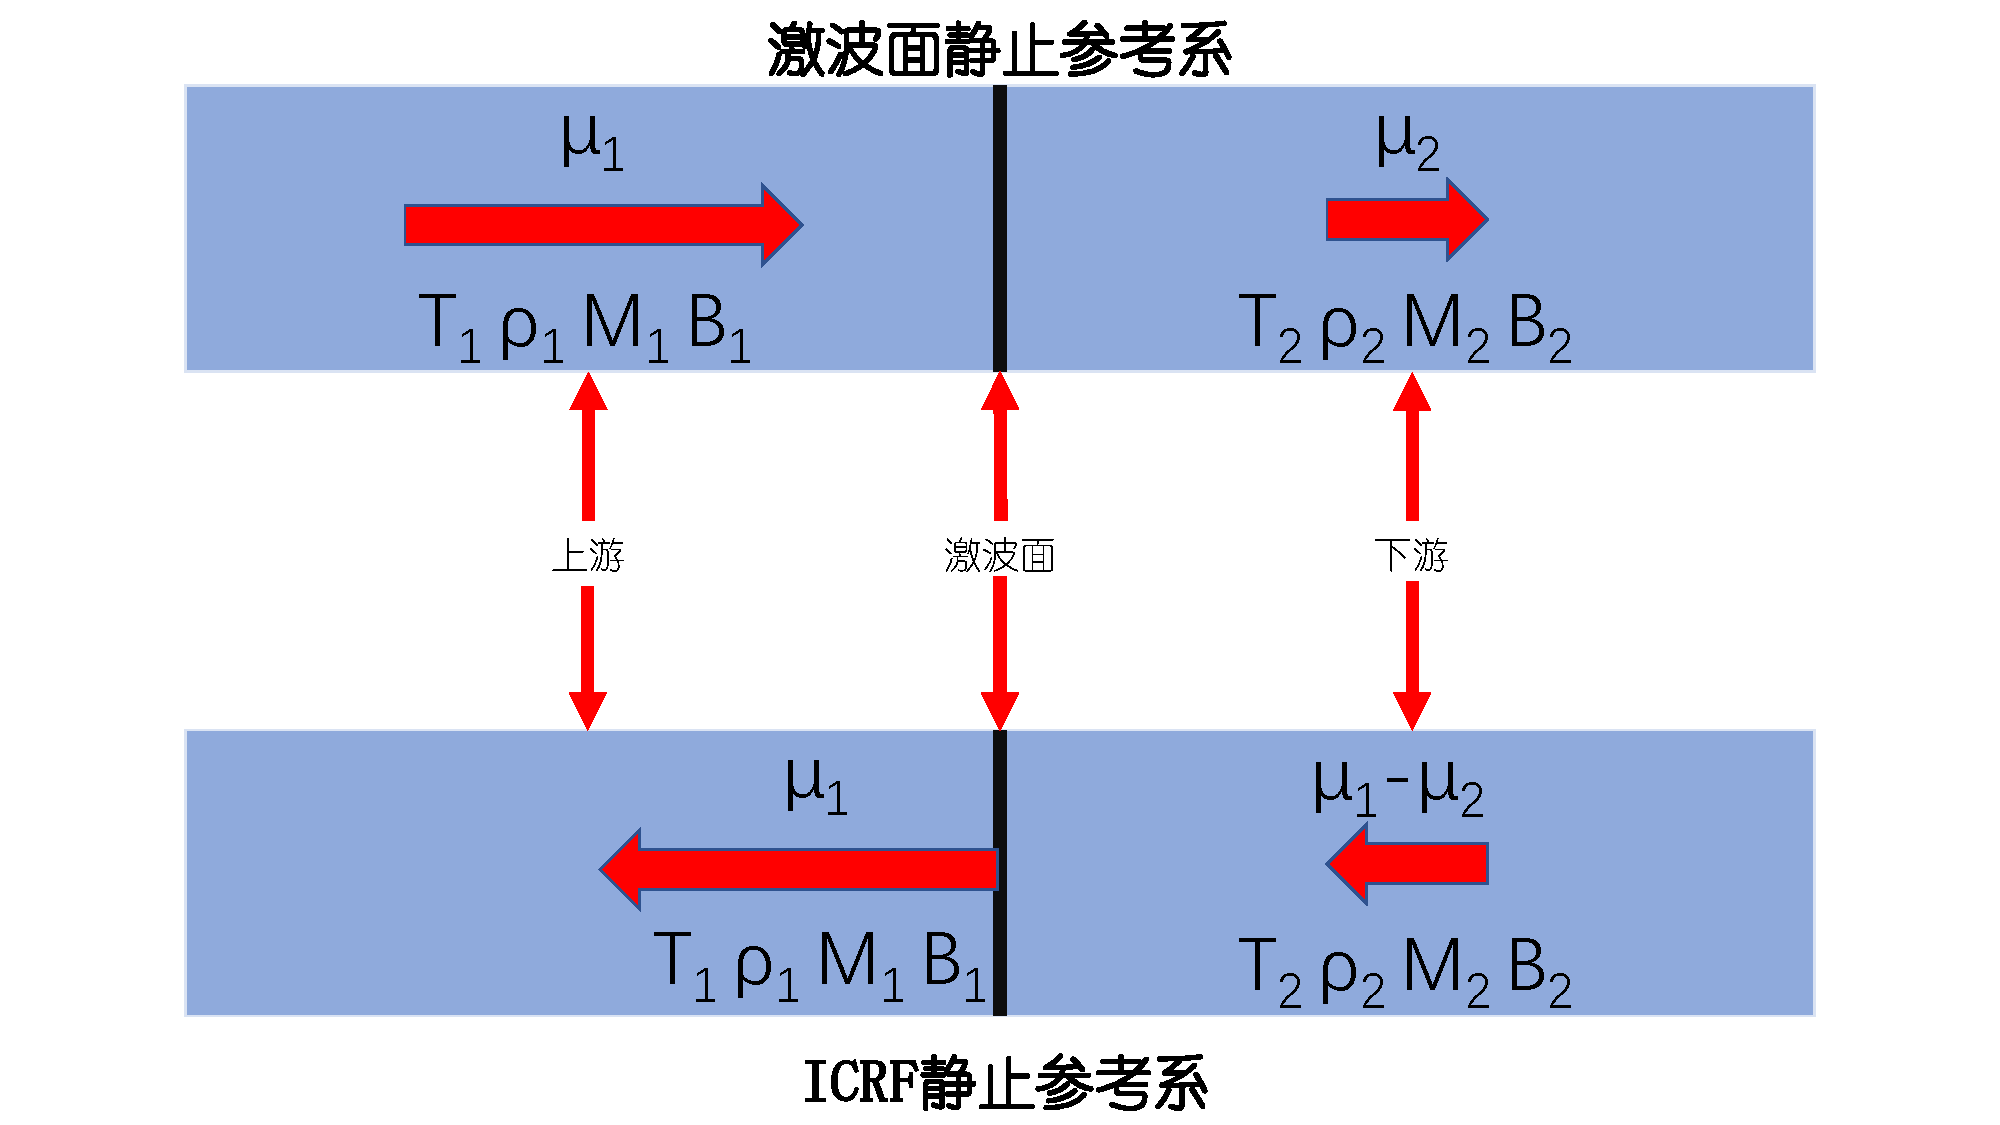
\includegraphics[width=0.9\textwidth]{ICRF.pdf}
    \caption{激波面静止参考系和国际标准参考系上下游的状态。}
\label{fig:shock}
\end{figure*}

而激波的重要特征之一就是,激波面分割开的上游和下游物理量差异很大,或者称为激波面不连续性。
取激波面为静止参考系,运动朝向激波面的为上游,速度、密度、温度、磁场、马赫数为$\mu_1$、
$\rho_1$、$T_1$、$B_1$、$M_1$,远离激波面的为下游,速度、密度、温度、磁场、马赫数为
$\mu_2$、$\rho_2$、$T_2$、$B_2$、$M_2$,如图~\ref{fig:shock}。
要注意,这里并没有抛射物混入,所以上下游其实都是原本就存在的ISM或者CSM,因而应该满足质量
守恒$\rho_1\mu_1=\rho_2\mu_2$,这里我们定义压缩比$r=\rho_2/\rho_1=\mu_1/\mu_2$。
而这里的动量守恒可粗略写为$\rho_1\mu_1^2=\rho_2\mu_2^2$,我们知道压强其实就是运动粒子
的动量造成的,这里的动量其实就是动压。
而热压在这里其实也是不可忽略的,所以准确的动量守恒方程应该为
$\rho_1\mu_1^2+p_1=\rho_2\mu_2^2+p_2$。
这里我们忽略了磁场,而遗迹当中磁压其实也很重要,考虑进来的话可得
$\rho_1\mu_1^2+p_1+B_1^2/8\pi=\rho_2\mu_2^2+p_2+B_2^2/8\pi$。
不过在这一节的讨论中,我们不考虑磁压,更多关于磁压的讨论请见章节~\ref{TheoryMHD}。


因为$c_{s}^{2}=\gamma p/\rho}$,故不考虑磁压的动量守恒方程改写为

\begin{equation}
  \begin{aligned}
    \rho_{1} \mu_{1}^{2}\left(1+\dfrac{p_{1}}{\rho_{1} \mu_{1}^{2}}\right)=
    \rho_{1} \mu_{1}^{2}\left(1+\dfrac{c_{s, 1}^{2}}{\gamma \mu_{1}^{2}}\right)=
    \rho_{1} \mu_{1}^{2}\left(1+\dfrac{1}{\gamma M_1^{2}}\right).
  \end{aligned}
\end{equation}

假设在国际标准参考系中(International Celestial Reference Frame,ICRF)激波上游介质在SNR
演化时标内可看作是静止的,如图~\ref{fig:shock},我们在激波面的静止系中看到的$\mu_1$
其实就是激波面本身的速度,$M_1$与$M$其实是一个量。
而$M\gg 1$,所以近似得$\rho_1\mu_1^2+p_1=\rho_1\mu_1^2$,
也就是$\rho_1\mu_1^2=\rho_2\mu_2^2+p_2$,两侧除以$\rho_2\mu_2^2$可得

\begin{equation}
    \begin{aligned}
       \dfrac{\mu_{1}}{\mu_{2}}=1+\dfrac{p_{2}}{\rho_{2} \mu_{2}^{2}}
       =1+\dfrac{1}{\gamma M_{2}^{2}} \ ,
    \end{aligned}
\end{equation}

如果取单原子气体绝热指数$\gamma$=5/3,可得$r=1+3/(5 M_{2}^{2})$。

能量守恒方程类似,$0.5\rho_1\mu_1^3+\rho_1\mu_1\epsilon_1+p_1\mu_1=
0.5\rho_2\mu_2^3+\rho_2\mu_2\epsilon_2+p_2\mu_2$,
理想气体中,$\epsilon=p/\rho/(\gamma-1)$,所以可得:

\begin{equation}
    \begin{aligned}
      \dfrac{1}{2}\rho_1\mu_1^3+\dfrac{\gamma}{\gamma-1}p_1\mu_1=
      \dfrac{1}{2}\rho_2\mu_2^3+\dfrac{\gamma}{\gamma-1}p_2\mu_2\ ,
    \end{aligned}
\end{equation}

同样因为$M_1\gg 1$,所以两侧除以$0.5\rho_2\mu_2^3$,可得$r^2=1+3/(M_{2}^{2})$。
与$r=1+3/(5 M_{2}^{2})$联立解方程组可得$r=4, M_{2}^{2}=0.2$。

激波上游主要是介质构成,而激波下游主要是受到SNR激波影响。
根据这个推导,我们可以通过介质和激波的性质,估计受到影响后的介质性质。
比如:

\begin{equation}
    \begin{aligned}
      \dfrac{1}{5}=M_{2}^{2}=\dfrac{\mu_{2}^{2}}{c_{s, 2}^{2}}=
      \dfrac{\mu_{1}^{2}}{16 c_{s, 2}^{2}}=\dfrac{\overline{m} \mu_{1}^{2}}{16 \gamma k T_{2}}\ ,
    \end{aligned}
\end{equation}

因而可得$k T_{2}=3/16 \overline{m} \mu_{1}^{2}$。
如果取H质量丰度为0.707,He质量丰度为0.274,其余粒子平均原子量为20,再考虑电子则平均粒子
权重为0.64。
则$\overline{m}$使用约化质量后得$k T_{2}=1.3 \times 10^{-6}(\mu_1/(km/s))^2 keV, T_2 =
15 (\mu_1/(km/s))^2 K$。
另外$p_2$和$\rho_2$也可以据此推出,这可以帮助我们理解很多SNR演化的细节,比如不同位置
的X射线辐射特征。

要注意,在这个推导过程中,我们用了很多假设:理想气体假设、强激波假设、介质静止假设、
单原子气体假设、无磁场假设。
这个无磁场假设是最有可能造成问题的,接下来我们要讨论DSA的核心部分,这一部分使用了上面
的推导结果,却又必须考虑磁场进行下一步分析。
问题是,我们下一步对磁场的讨论中,假设磁场对上面已经导出的结果影响不大。
可是实际上,在之前的推导过程中已经提到过磁场会影响动量守恒方程,当然,也将影响能量守恒方程。
不过,经典的DSA推导就是这么做的,所以我们也先接受这个简化模型。

之前的推导都是基于激波面静止坐标系,下面换个坐标系讨论。
设$\mu=\mu_1-\mu_2$,则
在上游静止坐标系中看,激波面的速度为$\mu_1$,下游速度为$\mu$,
在下游静止坐标系中看,激波面的速度为$\mu_2$,上游速度为$\mu$。
在上游静止坐标系中看,下游在朝上游移动,上游总会有一个相对上游静止的粒子来到下游。
之后,这个粒子与等离子体中的带磁场的团块(简称磁块)相互作用,这些团块其实是等离子体的集合体,
在上游静止坐标系中看以速度$\mu$朝上游运动。
而这个来到下游的粒子受到团块磁场偏转,类似于完全弹性碰撞,下游整体相对于粒子是质量极大
物体,根据完全弹性碰撞公式

\begin{equation}
    \begin{aligned}
      v_{small}^{\prime}=\dfrac{\vec{\bold{V}}_{small}\left(m_{small}-m_{large}\right)+2
      m_{large} \vec{\bold{V}}_{large}}{m_{large}+m_{small}}\ ,
    \end{aligned}
\end{equation}

粒子获得下游整体速度的两倍,然后来到上游。
这时候这个原本在上游静止坐标系中看来静止的粒子拥有了$2*\mu$的速度。
还是在上游静止坐标系中看,上游整体相对于粒子是质量极大物体,粒子以原速率反弹,也就是以
速度$2*\mu$进入下游。
类似于第一次循环,粒子获得下游整体速度的两倍,然后来到上游。
这时候这个原本在上游静止坐标系中看来静止的粒子拥有了$4*\mu$的速度。
平均每经过一次激波面,这个粒子就获得$\mu$的速度。
要知道,上游静止坐标系其实就是介质所在的坐标系,在SNR演化过程中基本可以认为就是静止,
所得的速度基本就是真实速度。
个人在将其中的粒子与磁块相互作用类比于完全弹性碰撞,细微之处或许略有不妥,但相对
来说简单理解,而推导结果也是没问题的。

虽然上游的粒子肯定会跑到下游,可是下游的粒子如果速度不够快,可能就追不上激波面,最终
远离加速区。
可实际上,经过一次循环加速,速度就达到了$2*\mu$,由$r=4$可知粒子速度已经远超过了下游速度,
所以基本不存在追不上激波面这种情况。
所谓逃逸的粒子多是由于磁场存在,在下游区域不断做回旋运动,虽然自身速度很高,但是
最终结果是随着下游整体在运动,而后慢慢脱离加速区。
所以说,下游粒子回到上游并不是因为自己速度很快,而是更类似于粒子扩散过程,这也是DSA
名称的由来。

经过讨论我们也发现,其实我们加速的粒子都是一开始周围介质的粒子,如前文所讲,超新星的抛射物
本身大部分没有参与到加速中。
当然我们在这里没有考虑反向激波,那又是另一个话题了。
所以下面要开展的能谱讨论里,我们只关注上游粒子。
此外,各种粒子实际上都有很高的初始速度,有一些甚至已经是相对论化的,直接根据上面定性
的推导计算获得的能量肯定不妥,所以要有更精确的计算。

设在上游静止坐标系上游粒子初始能量为$E$,初始动量为$p$。
考虑粒子经过激波面的入射方向与激波面法线夹角为$\theta$,而激波如果是相对论化的要再加一个
洛伦兹因子$\gamma_\mu$,这样,在下游静止坐标看这个粒子能量为
$E^{\prime}=\gamma_{\mu}(E+p \cos (\theta)\mu )$。
如果激波是非相对论的($\gamma_{\mu}=1$),而粒子是相对论化的($E=pc$),那么

\begin{equation}
    \begin{aligned}
      E^{\prime}=E+\dfrac{E}{c} \mu \cos (\theta)\ ,
    \end{aligned}
\end{equation}

从上游进入下游获得的能量就是

\begin{equation}
    \begin{aligned}
      \dfrac{\Delta E}{E} = \dfrac{\mu}{c} \cos (\theta)\ ,
    \end{aligned}
\end{equation}

反之亦然。

之前一直在讨论单个粒子,而能谱分布是相对很多粒子而言的。
假设不同方向粒子是均匀的,那么$\theta$到$\theta+d\theta$范围内的入射的粒子数与
$\sin(\theta)d\theta$成正比。
而很显然,垂直入射穿过激波面的概率为1,而平行入射几乎无法穿过激波面,那么粒子穿过激波面
的概率与$\cos(\theta)$成正比。
那么,如果有一群相同粒子之中,其中每一个都有可能以
$p(\theta)\propto \cos(\theta)\sin(\theta)d\theta$的概率穿过激波面。
总的穿过概率当然是1,那么有

\begin{equation}
    \begin{aligned}
      A \int_{0}^{\frac{\pi}{2}} \mathrm{d} \theta \cos
      (\theta) \sin (\theta) \equiv 1\ ,
    \end{aligned}
\end{equation}

解得A=2,所以$p(\theta)=2\cos(\theta)\sin(\theta)d\theta$。
这样总体粒子穿越一次激波面的平均能量获取就是

\begin{equation}
    \begin{aligned}
      <\dfrac{\Delta E}{E}>=\frac{2\mu}{c} \int_{0}^{\frac{\pi}{2}}
      d \theta \cos ^{2}(\theta) \sin (\theta) = \dfrac{2\mu}{3c} \ .
    \end{aligned}
\end{equation}

也就是说,粒子经过一次从上游到下游再回到上游,能量变为原来的$(1+4\mu/3c)$倍,
可见这是个一阶加速机制。

取$\beta_a=(1+4\mu/3c)$,而$P$为每个循环后仍留在加速区的可能性且为常数,设$N$为能量高于$E$的
粒子数,循环$k$次后可得

\begin{equation}
    \begin{aligned}
      N(>E)=N_{0} P^{k}\ ,\  E=E_{0} \beta_a^{k}\ .
    \end{aligned}
\end{equation}

取对数后相除得:

\begin{equation}
    \begin{aligned}
      \dfrac{\log \left(N(>E) / N_{0}\right)}{\log \left(E / E_{0}\right)}=
      \dfrac{\log P}{\log \beta_a} \ ,
    \end{aligned}
\end{equation}

也就是:

\begin{equation}
    \begin{aligned}
      N(>E)=N_{0}\left(\dfrac{E}{E_{0}}\right)^{\frac{\log P}{\log \beta_a}} \ ,
    \end{aligned}
\end{equation}

微分后可得:

\begin{equation}
  \label{eqn:SED}
    \begin{aligned}
      n(E) \propto E^{-1+\frac{\log P}{\log \beta_a}} \ .
    \end{aligned}
\end{equation}

这可以说就是一个幂律谱的能谱方程,可是我们目前不知道其谱指数,因为P还是未知量。
好在,我们知道每个循环中粒子逃逸的概率是(1-P),而这个概率是可以计算的。
设单位时间离开、进入加速循环的粒子数分别为$R_{out}$和$R_{in}$,则
$R_{out}/R_{in}=1-P$。
然后设$n$为加速区加速粒子的密度,如果密度均匀,则有:

\begin{equation}
    \begin{aligned}
      dn=\dfrac{n}{4 \pi} d \Omega \ ,
    \end{aligned}
\end{equation}

设粒子穿越激波面的速度为$v_p\cos(\theta)$,可得

\begin{equation}
    \begin{aligned}
      R_{i n}=\int_{u p \rightarrow d o w n} v_p \cos (\theta) d n =
      \dfrac{n v_p}{4 \pi} \int_{0}^{\frac{\pi}{2}} \cos (\theta) \sin (\theta)
      d \theta \int_{0}^{2 \pi} d \psi=\dfrac{1}{4} n v_p \ .
    \end{aligned}
\end{equation}

如果认为逃逸的粒子大部分来源于下游自然流出,那么$R_{out}=n\mu_2$。
也就是说$1-P=4n\mu_2/nv_p=\mu_1/v_p$,通常粒子入射速度很高,可以认为$\mu_1/v_p \ll 1$,
这说明大部分粒子都经过多次循环。
即使在介质区物质集体状态基本静止,单个粒子速度还是很快的,甚至大部分接近光速,可取$v_p=c$。
当然如果激波速度太快,而粒子初始速度太慢,那可能很快就被抛出加速区了。

目前为止,我们可以得到$P=1-\mu_1/c$,$\beta_a=(1+4\mu/3c)=1+\mu_1/c$。
再看方程~\ref{eqn:SED},其中

\begin{equation}
  \label{eqn:index}
    \begin{aligned}
        \begin{cases}
          \log P=\log \left(1-\dfrac{u_{1}}{c}\right) \sim-\dfrac{u_{1}}{c} \ , \\

          \log \beta_a=\log \left(1+\dfrac{u_{1}}{c}\right) \sim \dfrac{u_{1}}{c} \ , \\
        \end{cases}
    \end{aligned}
\end{equation}

然后可得

\begin{equation}
  \label{eqn:spec}
    \begin{aligned}
      n(E) \propto E^{-2} \ .
    \end{aligned}
\end{equation}

这就是由DSA机制刚好可得出的加速粒子幂律谱,是一个非常棒的结果,一经提出便被广泛认为是
SNR中产生同步辐射的相对论电子的基础。
当然我们不要忘了这个计算结果其实是基于很多假设的。
在推导激波及上下游性质时,我们已经提到了一些假设。
而在推导粒子加速时,我们又引入一些新的假设:弹性碰撞假设、激波非相对论假设、粒子相对论化
假设、粒子各向同性假设、非线性效应可忽略、忽略其它逃逸方式。
每一个假设不成立,都会导致谱指数的改变。
比如经常出现激波并不是强激波,那么$r\neq4$,结果只能用
$P=1-4\mu_2/c$,$\beta_a=(1+4\mu/3c)\neq1+\mu_1/c$。
类似方程~\ref{eqn:index},可得

\begin{equation}
    \begin{aligned}
      n(E) \propto E^{-\frac{r+2}{r-1}} \ .
    \end{aligned}
\end{equation}

可见激波越弱,谱指数越大,谱越陡。
另外,磁场的存在也会使得谱指数变大,具体推导见章节~\ref{TheoryMHD}。
同时,周围介质其实并不一定是静止的,比如前身星本身有高速运动,那么相当于介质存在一定速度,
这样SNR不同方向激波中的加速效率$\beta_a$也是不一样的,这也是SNR壳层亮度不同的一个原因。

此外,我们在这里都是忽略了辐射损耗的,然而,高效的激波加速会导致更严重的辐射损耗。
同时,大量的高能相对论粒子会缩小绝热系数$\gamma$。
这两个效应都可能增大压缩系数$r$\citep{Ellison2005},而且相关观测也发现SNR中有的位置
压缩系数可能被增大\citep{Voelk2007}。
这些条件会使得谱指数变小,谱变平,最终我们看到的粒子分布是各种效应叠加的结果。



\subsection{宇宙线起源}
自从\citet{hess1912beobachtungen}发现宇宙线以来,这一领域一直受到人们的广泛关注,而
对其起源的猜测也从未间断\citep{Reynolds2008a}。
不过,随着近几年高能观测的增多,SNR对银河系宇宙线有很大贡献已经成为一个不争的事实
\citep{Ackermann2013, Joubert2016, Jogler2016}。
当然诸如脉冲星风云(Pulsar Wind Nebula, PWN)和黑洞的贡献应该也需要考虑
\citep{Abeysekara2018, Profumo2018}。
不过,测量的宇宙线能谱,在考虑传播过程后需要一个能产生谱指数为-2的幂律分布
粒子的机制来解释,虽然SNR刚好满足这一条件,但其实我们推导的DSA产生的能谱只是加速区的能谱,
加速区中的粒子释放到ISM中的时候会经历冷却、或者反向激波再加速等过程,最终的谱指数很可能
不是-2。
所以说,我们对宇宙线能谱仍然不甚了解,除了这个粒子释放的问题,还有一直难以理解的“膝区”
\citep{Hoerandel2003}。
而对其解释其实有很多,很自然的想法就是加速源有两种,加速产生的能谱不同。
但具体这两种是什么,会不会多种的贡献互相叠加,我们还不是很清楚。

我们可以先尝试了解SNR对宇宙线能谱的贡献\citep{Ptuskin2010},这样我们不仅需要
知道其谱指数,还需要得到能谱阶段能量,也就是SNR能将例子加速到的最大能量$E_{\max}$。
这个也可以由DSA来估计。
我们知道下游粒子来到上游再回到下游这个循环中,其实主要影响粒子宏观运动的是扩散效应。
这里引入扩散系数$D$,假设粒子从下游进入上游后,跑了$t_d$的时间到达距激波面最远处,然后
与追上来的激波面接触并进入下游,这个最远处与激波面距离为$l_d$,可得
$l_{d} \approx \sqrt{D t_{d}}$。
当然,我们也有$l_{d}=u_{1} t_{d}$,解得$t_d \approx D/\mu_1^2$。
扩散系数其实是与粒子的能量有关的$D=D_{0} E^{\alpha}$,能量越大,扩散系数越大,
而$l_{d}$、$t_{d}$也就越大,多次加速后会超出加速区范围。
这其实是另一种粒子逃逸方式\citep{Li2012},但相比于直接从下游流走的粒子数要少,所以在
DSA推导时没有考虑。

这里可见,一次循环的加速时标近似于$t_{d}$,假设最多可经历$m$次循环,那么所得最高能量为
$E_{\max }=(u_{1}^{2} m t_{d}/D_{0})^{1/\alpha}$。
根据类似思路,\citet{1983A&A...125..249L}估算出SNR最多能加速粒子到100TeV,而膝区位置
都是大于1PeV的,这个$E_{\max}$远远不够。
\citet{Zirakashvili2018}将磁场考虑在内,并尝试加入一个前身星星风吹出的壳层来放大初始
介质磁场,从而提高截断能量。
而我们也尝试通过模拟来检验这件事,并证实了这种思路的可行性\citep{Zhang2018}。
不过,目前对这个模型的观测支持其实并不多,因为我们观测到遗迹时其前身星星风早已被激波
冲散,很难得到直接证据,或许对年轻的遗迹周边进行观测能够帮助我们确切证实这件事。

\subsection{SNR中的辐射机制}

除了很早就有人意识到的DSA加速的电子会产生同步辐射,且射电谱指数$\beta$与电子分布谱指数$\eta$
存在关系$\beta=(\eta-1)/2$,
\citet{Reynolds1981}提出类似的机制也可以产生非热的X射线辐射,而他们发现SN 1006
就是一个很好的例子\citep{Becker1980},可是这要求粒子加速能量远超过100TeV,
在当时来看是不太可能的。
后来,\citet{1982ApL....22..103G}接近1keV的能段发现了X射线的谱线,所以大家都认为
SN 1006也是热谱,无法作为产生X射线非热谱的例子。
然而,更高空间分辨率的观测显示,这个SNR壳层区的确是非热的,中心区才是有谱线的
\citep{Koyama1995},所以事情又反转了。
后来,\citep{Reynolds1998}通过改进自己之前的模型,发现即使粒子截断能量在100TeV也能
很好拟合SN 1006的X射线能谱。
这个工作说明了两件重要的事情,DSA产生的相对论电子的确可以通过同步机制产生X射线非热辐射,
同时可知,DSA的确可以将粒子加速到100TeV,我们对DSA的推导是正确的。

除了主要产生同步辐射的高能电子,稍微低能一些的非热电子会通过韧致辐射产生能量范围从keV
到TeV的光子。
所有电子都会通过与各种原子核相互作用产生韧致辐射。
热电子只会产生一般的热连续谱辐射,而能量较高的非热电子则通过同步辐射产生幂律谱的同时
也会通过韧致辐射产生幂律谱。
通常一个能量为$E$的电子经过韧致相互作用会释放能量大约为$E/3$的光子,可是同步辐射并不会
有这么高的能量转化,结果就是能量为TeV的电子,可能通过韧致辐射产生TeV光子,但通过同步
辐射只能最高产生keV的光子。
另外,其实如果电子能量很高,互相之间也会产生韧致辐射,有时在拟合能谱时是不可忽略的。

高能电子本身会散射背景光子场,比如宇宙微波背景辐射(Cosmic Microwave Background,
CMB),然后产生能量能达到TeV的光子,这就是逆康普顿散射。
背景场可能有很多种,SNR自身产生的射电辐射、星系自身的背景辐射等有所贡献。
真正在拟合能谱时,甚至要考虑附近大质量恒星的辐射。

此外,高能质子相互作用可能产生$\pi^0$介子,$\pi^0$介子衰变成的$\gamma$光子能量也很高。
不过这种情况在SNR本身的环境中很难发生,因为这要求很高的质子密度。
而当SNR周围刚好存在分子云,激波与分子云相互作用时就会产生非常不一样的能谱。
之前观测上已经有很多证据表明电子在SNR中被加速至高能,但是这些其实无法说明质子是否也被加速。
可我们观测到的宇宙线主要由质子组成,电子因为磁场偏转无法到达地球,宇宙线的能谱也主要也是由
质子所贡献。
所以说,观测到质子在SNR中加速才能说明SNR是宇宙线的起源地。
而通过观测激波与分子云相互作用时产生的与电子辐射的不同的能谱,我们可以确定的确有高能质子
的存在,这才真正证实SNR是部分宇宙线的来源地。



\section{磁流体模拟基础}
\label{TheoryMHD}

\subsection{磁场的重要性}
前述DSA的推导中我们都忽略了磁场,不然动量守恒方程应该是
$\rho_1\mu_1^2+p_1+B_1^2/8\pi=\rho_2\mu_2^2+p_2+B_2^2/8\pi$。
现在我们来讨论一下,磁场是不是真的不重要。
取$\rho_1=1 m_p cm^{-3}, \mu_1 = 100 km/s$,则动压
$\rho_1\mu_1^2=1.6 \times 10^{-10} dyn/cm^{2}$。
取$\B_1=9\mu G$,则磁压$B_1^2/8\pi=3.2 \times 10^{-12} dyn/cm^{2}$。
这里我们用的速度是比较小的,而磁场是比较大的。可见,磁压相对来说不重要。
不过磁场在激波与介质作用时是会放大的,我们算过压缩比$r=4$,因为磁通守恒,我们暂且
假设激波后磁场放大4倍,那么取$B_2=36\mu G$,则磁压
$B_2^2/8\pi=5.1 \times 10^{-11} dyn/cm^{2}$。
这时候磁压都达到了动压的一半,不应该忽略了。
其实考虑湍流后磁场放大到$100\mu G$现在看来已经是可能的了\citep{Ji2016b},假设放大十倍
后可取$B_2=90\mu G$,则磁压$B_2^2/8\pi=3.2 \times 10^{-10} dyn/cm^{2}$。
所以,下游的磁压其实是不能忽略的。
如果上游的磁场因为前身星星风等原因得到放大,也就不应该忽略。
总体来说,大部分情况是不能忽略磁压的,故经典DSA是存在这样一个明显的瑕疵的。

那么磁压到底对我们的DSA推导影响多大呢?
类似于DSA推导,设激波后磁场放大4倍,即$B_2=4B_1$,将考虑磁场的动量守恒方程两侧除以
$\rho_2\mu_2^2$,可得

\begin{equation}
    \begin{aligned}
      \dfrac{\mu_1}{\mu_2} = 1+\dfrac{p_2}{\rho_2\mu_2^2}+
      \dfrac{15}{16\rho_2\mu_2^2}\dfrac{B_2^2}{8\pi }\ ,
    \end{aligned}
\end{equation}

然后设热压磁压比$\beta_b=8\pi p/B^2$,可得

\begin{equation}
    \begin{aligned}
      r = 1+
      \left(1+\dfrac{15}{16\beta_{b,2}}\right)\dfrac{3}{5 M_2^2} \ .
    \end{aligned}
\end{equation}

类似的,已知能量守恒方程为

\begin{equation}
    \begin{aligned}
      \dfrac{1}{2}\rho_1\mu_1^3+\dfrac{\gamma}{\gamma-1}p_1\mu_1+\dfrac{\mu_1B_1^2}{8\pi}=
      \dfrac{1}{2}\rho_2\mu_2^3+\dfrac{\gamma}{\gamma-1}p_2\mu_2+\dfrac{\mu_2B_2^2}{8\pi}\ ,
    \end{aligned}
\end{equation}

两侧除以$0.5\rho_2\mu_2^3$,整理可得

\begin{equation}
    \begin{aligned}
      r^2 + \dfrac{3r}{40\beta_{b,2}M_2^2} = 1 + \dfrac{3}{M_2^2}
      +\dfrac{6}{5\beta_{b,2} M_2^2} \ .
    \end{aligned}
\end{equation}

联立动量守恒方程,解得

\begin{equation}
      \label{eqn:ratio}
    \begin{aligned}
        \begin{cases}
          M_2^2 = \dfrac{1}{5}+\dfrac{2}{5\beta_{b,2}}+\dfrac{1131}{256\beta_{b,2}^2} \ , \\

          r = 1 + \dfrac{3}{5M_2^2}\left(1+\dfrac{15}{16\beta_{b,2}}\right) \ . \\
        \end{cases}
    \end{aligned}
\end{equation}

可见,热压相比磁压越大,磁场部分就越不重要,最后可以回到经典DSA推导。
要注意,我们在这里直接设激波后磁场放大4倍,如果我们认为这个倍数就是压缩比$r$,那么将其
代入后$B_2=rB_1$,根据相同步骤也可推导出更准确的结果。
不过这样推导过于复杂,而且真实情况中,磁场放大机制不止介质压缩,各种不稳定性及局部湍流
都会影响放大,所以这里暂且使用这一粗略结果。

同时,$\beta_{b,2}\to \infty, r\to4$,分析可知,$r$在这里最大为4,其实即使考虑
激波后磁场放大$r$倍,计算结果也是最大为4,也就是说压缩比在强激波条件下为最大。
再与方程~\ref{eqn:spec}相比较,可知考虑磁场后的激波产生的幂律谱会更陡,不能算是强激波,
看似好像这个激波是弱的,更难将粒子加速到高能。
可实际上,粒子在强磁场中更容易驻留,同样时间内经历更多次加速循环,因而虽然谱陡,但是
加速到高能的粒子反而可能更多。
当然,这需要进一步计算,类似应用请看\citet{Zirakashvili2018}的工作。
而这个推导也可以帮助我们理解“膝区”形成,可能证实因为有的激波加速磁场很强,而有的很弱导致
谱指数的不同。
磁场很强的激波加速中,截断能量更高,可是谱很陡,而磁场很弱的激波加速正相反。
也就是说强磁场激波加速对高于“膝区”的谱贡献大一些,而弱磁场激波加速对低于“膝区”的谱贡献
大一些。
此外,这种因为磁场强度不同而导致的粒子谱指数变化自然地也会影响到同步辐射谱指数,而实际上
SNR不同区域的谱指数相差很大\citep{Leahy2005, Tian2005},我们这里讨论的因素应该也对这
一现象有很大影响。

总之,磁场对SNR的演化及粒子的性质影响很大,我们不应该将其忽略,这也是我们开始这篇文章中
工作的重要原因之一。

\subsection{磁流体特性}
说到流体,我们要提到一个最著名的假设,连续介质假设。
当我们讨论流体时,通常都默认这一假设成立,但是在某些极端情况,尤其是天文研究中,这个假设
很多时候都是不成立的。
这个假设主要就是说流体中的组成粒子都可看作质点,质点间几乎不存在间隙。
不过实际判定的标准分为空间和时间两个方面,这两个方面都是对我们统计粒子这一行为提出的。

首先,空间上,进行统计的粒子可看作质点,微观上足够大,宏观上足够小。也就是说,微观上粒子
尺度比粒子间空隙大得多,宏观上粒子比所研究的尺度小得多。比如研究倒一杯水,水分子比水分子
间空隙要大,杯子的尺度比水分子的尺度要大。
而时间上,进行统计粒子用的时间,在微观足够长,在宏观上足够短。也就是说,微观上时间够长,
粒子已经碰撞多次满足统计要求,而宏观上时间够短,统计粒子的时间比我们研究流体过程时间
要短。

说到这里,我们大概意识到,SNR的磁流体模拟其实是不满足连续介质假设的,主要是因为粒子间空隙
比粒子大得多。
不过,很多时候SNR中的流体是可以看作连续的,因为我们进行统计粒子用的时间甚至可以以年为单
位计算,这时候粒子间已经碰撞多次,统计上可以当作空隙很小。
其实,我们在推导DSA使用守恒方程时,已经默认了这一假设成立。
举个例子,研究时间很短,上游粒子来到下游,还没有其它粒子回到上游,这就导致统计粒子
的时间比我们研究流体过程时间要长,这时候守恒律当然是不成立的。
一般情况下,这一假设没有问题,不过要做极端讨论时就得考虑。

此外,在SNR演化过程中会存在各种不稳定性,
其中明显会出现的就是瑞利-泰勒不稳定性(Rayleigh-Taylor instability, RTI),这种
不稳定性主要发生在密度高的流体与密度低的流体相向接触时互相之间存在加速度时,看起来很明显
超新星爆发的抛射物与介质之间的关系就是这样。
不过要注意的是,这种不稳定性是需要持续施力的,一旦没有加速度,我们看到的参数起伏就不再
是RTI直接导致的,而是初期RTI的扰动引起的连锁反应。
所以对于大部分SNR如果中心有PWN的持续供能,那么RTI会持续起作用,如果没有,可能RTI只是
剩下后续的扰动影响。
特别的是,RTI尤其要与里克特迈耶-梅什科夫不稳定性(Richtmyer–Meshkov instability, RMI)
区分开,这种不稳定性是在两种流体接触的位置因为局部扰动引起瞬间加速导致的,我们在磁流体
模拟中遇到的更多是这种不稳定性。
此外,与RTI看起刚好相反的是开尔文-亥姆霍兹不稳定性(Kelvin–Helmholtz instability, KHI),
两种流体相切接触时才会产生KHI。
虽然看起来SNR中抛射物与介质是相向接触,但实际上,因为介质密度不均匀,相切接触也是时有发生。
这些不稳定性都会导致局部参数的起伏,放大局部磁场,改变不同区域同步辐射谱指数,这才导致
我们看到的SNR内部结构千变万化。

此外,我们在推导DSA时只是研究了二维情况,三维的守恒方程要考虑更多,而且引力也是可以考虑
在内的,这里我们给出实际在磁流体模拟中使用的方程:

\begin{equation}
\frac{\partial}{\partial t} \left( \begin{array}{c}{\rho} \\ {m} \\ {E+\rho \Phi}
\\ {B}\end{array}\right)+\nabla \cdot \left( \begin{array}{c}{\rho v} \\
{m v-B B+\mathbf{I} p_{t}} \\ {\left(E+p_{t}+\rho \Phi\right) v-B(v \cdot B)}
\\ {v B-B v}\end{array}\right)^{T}=\left( \begin{array}{c}{0} \\
{-\rho \nabla \Phi+\rho g} \\ {m \cdot g} \\ {0}\end{array}\right)
\end{equation}

其中$\mathbf{I}$是单位积,
$\mathbf{I} \equiv \hat{\boldsymbol{e}}_{1} \hat{\boldsymbol{e}}_{1}+
\hat{\boldsymbol{e}}_{2} \hat{\boldsymbol{e}}_{2}+\hat{\boldsymbol{e}}_{3}
\hat{\boldsymbol{e}}_{3}$, 而${m}=\rho {v}$,$p_{t}=p+B^{2} / 8\pi$,
$E=\rho \epsilon+m^{2}/2 \rho+B^{2}/8\pi$,$\rho \epsilon=\rho \epsilon(p, \rho)$,
$\Phi$和$g$是引力势和加速矢量。
我们之前对DSA的讨论是基于二维的,三维磁流体中需要考虑磁场张量作用,在方程中体现为$BB$等
并矢。
这种张量作用会产生阿尔文波,这种波是带电粒子在垂直于磁场方向运动时,受到局部扰动时产生的
沿着磁场方向运动的波,这种波会影响局部磁场,导致不同位置的粒子加速情况有所不同,与上面
提到的三种不稳定性一起改变不同区域同步辐射谱指数。
因为我们实际进行的磁流体模拟是三维的,所以在程序编写中是对其有所考虑的。
当然,我们之前的讨论也忽略了引力,这个忽略与忽略磁场不同,对SNR来说是非常合理的。
此外,虽然我们这里的方程写得很正确,但是数值计算时可能依旧会有问题,比如磁场无源其实就
无法保证,因而与物理事实其实还是有些差别。
不过经过改进算法,我们可以克服这些问题。
